\setcounter{page}{1}
\begin{center}
\xiaosihao
\textbf{一种简单的ECG噪声检测与分类方法——适用于可穿戴ECG监测设备\\}
~~\\
~~\\
\wuhao
\noindent
\begin{minipage}{\linewidth}
\textbf{摘要:}
\kaishu
对心电图(Electrocardiogram,ECG)信号质量的评估是大多数Holter ECG信号和动态ECG信号分析应用中的第一步,也是不可或缺的一步。本文提出了一种简单的检测并分类ECG噪声的方法,这种方法由四个主要步骤组成:滑动平均滤波,分帧,特征提取和多级决策树算法。该方法提取了每帧信号中的动态振幅范围和最大自相关峰等特征。在第一级决策中,使用一个具有波幅依赖性的决策规则来检测低频噪声(包含基线漂移(Baseline Wander, BW)和突变干扰(Abrupt Change, ABC))以及高频噪声(包含工频干扰(Power Line Interference, PLI)和肌电干扰(Muscle Artifacts, MA))。在第二级决策中,该方法根据信号的局部动态振幅范围,进一步将低频噪声归类为BW噪声或ABC噪声,根据信号的局部最大自相关峰将高频信号分为PLI噪声和肌电干扰。我们使用了多种不同受干扰程度的ECG信号测试了该检测分类方法。结果表明,本方法的平均灵敏度可达97.88\%,效率可达91.81\%,精确度可达89.06\%。
~~\\
\end{minipage}
\end{center}

\wuhao
\section{简介}

近年来,可穿戴式心脏保健监测让我们能够不间断地记录ECG信号,并使心血管疾病得到尽早地发现和治疗。一般来说,常见的ECG信号振幅为10$\mathrm{\mu}$V至5mV,而其频率介于0.05-150Hz之间。ECG信号记录普遍受到噪声干扰,即基线飘移,工频干扰,肌电干扰以及设备噪声干扰。另外,运动伪影干扰在基于无线体域网(WBANs)的ECG监测中也十分普遍。从图1所示的受干扰ECG信号中,我们可以注意到BW,PLI以及肌电干扰造成了ECG特征点、特征测量、心率分段等项目的测量不准确。因此,ECG信号质量评估已成为大多数Holter ECG信号和动态 ECG信号分析应用中的第一步,同时也是不可或缺的一步,这些应用包括心律失常识别、心率变异分析、基于ECG的生物特征识别、每搏心跳间血压的不间断测量以及睡眠呼吸暂停检测等。另外,信号质量评估不仅显著提高了心血管疾病诊断系统的准确性,也能帮助我们挑选出适当的ECG信号增强技术。然而,可穿戴ECG监测设备虽然保证了信号的持续纪录以及心脏疾病的提早发现,但其电量、电池寿命、计算能力和存储器大小均为有限。所以,在选择适当的噪声削减技术时,可穿戴设备需要的是低耗能的噪声检测和分类手段,并借此保证所记录的ECG信号的临床可接受性。

\subsection{对ECG信号质量评估方法的回顾}

根据相关研究报告,多数信号质量评估(Signal Quality Assessment, SQA)方法均基于如平均数、标准差、峰度及启发式规则的统计特性。在参考文献4中,Orphanidou等人提出了针对QRS信号和PPG(PhotoPlethysmoGraphy)信号的一种信号质量衡量方法:先使用启发式规则检测QRS或PPG脉冲中提取出的特征、RR间期、最大和最小RR间期的比值,再进行模板匹配。参考文献5提出了一种通过人工重建目标导联来评估信号质量的方法,其步骤包括LF与HF噪声移除、能量下凹指数分析、使用神经网络程序估算出ECG导联间的相关性。参考文献6中,L. Johannesen和L. Galeotti等人提出了一种自动为ECG质量评分的方法。这种方法通过分析导联丢失、检测QRS波、对QRS波分割、检测错误的QRS波来排除ECG中的宏大误差,再对BW、PLI和肌电干扰加以量化。在参考文献7中,D. Hayn等人提出了基于QRS检测的ECG质量评估标准,其中包括对空载导联的检测,尖峰检测,导联信号交叉点检测以及QRS检测的鲁棒性。

\begin{wrapfigure}{r}{24em}%靠文字内容的左侧
\label{figNo.1}
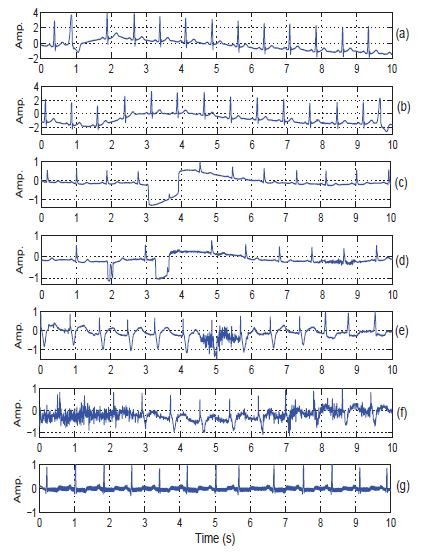
\includegraphics[width=0.6\columnwidth]{fig1.jpg}
\caption{
\wuhao
图中的ECG信号掺入了不同类型的噪声及伪影:(a)和(b)中ECG信号受基线漂移影响,(c)和(d)中ECG信号受突变干扰,(e)和(f)中ECG信号受肌电干扰,(g)中ECG信号受PLI噪声干扰。
}
\end{wrapfigure}
参考文献8中提出了一些用于确定临床可接受性的信号质量指标和数据融合方法,包括谱能分布、高阶矩、通道间和算法间协议、多层神经网络和支持向量机。文献9中提出了一种使用经验模态分析和统计学方法来自动探测运动伪影和噪声干扰的方式。文献10中Hayn等人提出了针对移动医疗应用中患者增权的ECG质量评估方法。这种方法分析了信号的基本特征(振幅,尖峰,常数信号部分等)、不同导联间的交叉点个数以及QRS振幅与噪声振幅的比值。文献11中B.E.Moody提出了一种基于条件的ECG信号质量控制。文献12提出了一种基于Android平台的ECG质量评估,能够探测所有导联中的失效导联、全局高频噪声、造成QRS探测问题的含噪声导联、全局低频噪声以及窦性搏动中的高低频噪声。文献13中,Liu等人提出了使用手机处理所收集的ECG数据的实时信号质量评估方法。这种方法能够通过检测四种标志性事件来判别四种错误:电极的错误放置,强脉冲,强高斯噪声和基于模版匹配的R波波峰探测算法造成的错误。通过对这四种标志性事件的检测,该方法能分别计算出单个导联的单一信号质量指数和12个导联的整体信号质量指数。文献14提出了Android平台上评估ECG信号质量的简易评分系统。文献15中提出了一种评估正常状态和噪声所致衰减的动脉血压信号质量指数。大多数现有的方法都使用了PICC2011(Physionet/Computing in Cardiology Challenge 2011)所提供的数据。


\subsection{现有SQA方法的局限性}
许多基于QRS信号检测的SQA方法都源于对输入ECG信号中探测到的RR间期的分析。当无噪声ECG信号记录包含以下成分时,RR间期的精确测量将收到严重干扰:(1)宽QRS波群;(2)低振幅QRS波群;(3)负极性的QRS波群;(4)RR间期中的突变;(5)QRS波的振幅突变;(6)QRS波形态的突变;(7)尖锐的P波和T波。在这些情况下,现有的使用心率评估ECG信号质量的方法要求能够对ECG信号中出现的R峰进行精确的实时测量。大多数方法采用传统的R峰检测(或波形描绘)算法,这些算法应用于ECG信号时检测率很低。此外,大多数检测方法包含了一系列用于检测R峰的振幅阈值、持续时间阈值和间期长度阈值,这些阈值要么忽略了噪声,要么计入了噪声,最后错过了R峰。一种包含适当的振幅阈值和时间阈值的前向搜索算法被广泛应用于采纳或抛弃$t_{m}$和$t_{n}$之间已检测到的R峰:(1)$t_{n}-t_{m}<0.2 s$(不应期);(2)$t_{n}-t_{m}>1.5RR_{avg}$时向前搜索。这些条件或许能提高对于规律性节律的探测,但其中一些条件可能相互冲突。此外,前向搜索机制在检测含有变化QRS波群的非规律性节律时不能被终止。还有,启发式规则中往往含有大量阈值设定。大多数方法中,这些用于检测的阈值是基于之前检测到的R峰设定的。这样,检测方法的性能就极大地依赖于对学习阶段中初始阈值的估计是否精确。

基于EMD的方法将局部波形中的ECG信号和噪声分离成一系列固有模态函数方程(Intrinsic Mode Functions, IMFs)。这时,从信号IMF中确定出噪声IMF就很困难。虽然每一个小波子带的频率范围是已知的,但BW、PLI、MA所致噪声以及ECG信号的小波系数被分入了细节子带和近似子带中。因此,在PQRST波的形态和噪声的特点均随时间变化时,噪声子带的特征难以确定。然而,我们并不能纠正小波滤波器、分解层数和特征子带,因此建立一种低复杂度的ECG信号质量自动评估方法仍然是一个具有挑战性的研究课题。


\subsection{本文的贡献}

本文提出了一种简单直接的ECG噪声监测和分类方法。我们提出的方法分为四个主要步骤:滑动平均滤波,分帧,特征提取和多级决策分类。该方法中,一些如全局/局部动态振幅和最大自相关峰等特征被提取出来。在这些特征的基础上,多级决策被建立起来并用于自动检测和分类ECG噪声。实验结果表明该方法在检测各种不同类型的带噪/非带噪信号时的分类准确性均为可接受的。
本文的组织结构介绍如下:第二部分描述了所提出的ECG噪声检测和分类方法;第三部分介绍了使用多种带噪/非带噪ECG信号测试并验证所提出方法的性能。最后,第四部分得出了结论。